\documentclass[12pt]{article}
\usepackage[a4paper, margin=2.5cm]{geometry}
\usepackage[utf8]{inputenc}
\usepackage[T1]{fontenc}
\usepackage{setspace}
\onehalfspacing
\usepackage{graphicx}
\usepackage{amsmath, amssymb}
\usepackage{booktabs}
\usepackage{caption}
\usepackage{float}
\usepackage{hyperref}
\hypersetup{hypertexnames=false}
\usepackage{pgfplots}
\usetikzlibrary{intersections, patterns, decorations.markings, calc}

\newcommand{\E}{\mathbb{E}}
\newcommand{\Var}{\mathrm{Var}}
\newcommand{\Cov}{\mathrm{Cov}}
\newcommand{\Info}{\mathcal{I}}

\begin{document}

% ═══════════════════════════════════════════════════════════════════════════════
% FRONT PAGE
% ═══════════════════════════════════════════════════════════════════════════════
\begin{titlepage}
\centering
\vspace*{1.5cm}
{\LARGE\bfseries Econometrics II --- Portfolio Exam}\\[0.5cm]
{\Large Spring 2026}\\[1.5cm]
{\large Exam Number: [92 \& XX]}\\[1.5cm]
\begin{tabular}{ll}
\toprule
\textbf{Part} & \textbf{Character Count} \\
\midrule
Part 1 & 10,105 characters \\
Part 2 & 11,044 characters \\
Part 3 & No character limit \\
\bottomrule
\end{tabular}

\vspace{1.2cm}

{\large\bfseries Individual Contributions}\\[0.3cm]
{\small Number of students in group: 2}

\vspace{0.4cm}
\begin{small}
\begin{tabular}{@{}p{1.6cm} p{13cm}@{}}
\toprule
\textbf{Exam no.} & \textbf{Responsible for sections/chapters} \\
\midrule
XX &
\textbf{P1:} \S\ref{sec:p1-theory} Econometric Theory.\;
\textbf{P2:} \S\ref{sec:p2-data} Data; \S\ref{sec:p2-empirical} Empirical Analysis.\;
\textbf{P3:} \hyperref[sec:p3-q2]{Q2}; \hyperref[sec:p3-q4]{Q4}; \hyperref[sec:p3-q6]{Q6}; \hyperref[sec:p3-q7]{Q7}. \\[4pt]
92 &
\textbf{P1:} \S\ref{sec:p1-data} Data; \S\ref{sec:p1-empirical} Empirical Analysis.\;
\textbf{P2:} \S\ref{sec:p2-theory} Econometric Theory.\;
\textbf{P3:} \hyperref[sec:p3-q1]{Q1\,(a--c)}; \hyperref[sec:p3-q3]{Q3}; \hyperref[sec:p3-q5]{Q5\,(a--b)}. \\[4pt]

\midrule
92 \& XX &
\textbf{Collaborative:} P1 \S\ref{sec:p1-intro} Intro, \S\ref{sec:p1-discussion} Discussion, \S\ref{sec:p1-conclusion} Conclusion;\; P2 \S\ref{sec:p2-intro} Intro, \S\ref{sec:p2-discussion} Discussion, \S\ref{sec:p2-conclusion} Conclusion. \\
\bottomrule
\end{tabular}
\end{small}
\vfill
\end{titlepage}

% ═══════════════════════════════════════════════════════════════════════════════
% PART 1 — Forecasting Economic Growth and Growth-at-Risk
% ═══════════════════════════════════════════════════════════════════════════════
\part{Part 1 --- Forecasting Economic Growth and Growth-at-Risk}
\setcounter{section}{0}
\setcounter{figure}{0}
\setcounter{table}{0}
\setcounter{equation}{0}
\renewcommand{\thefigure}{1.\arabic{figure}}
\renewcommand{\thetable}{1.\arabic{table}}
\renewcommand{\theequation}{1.\arabic{equation}}

% ─────────────────────────────────────────────────────────────────────────────
\section{Introduction}\label{sec:p1-intro}
% ─────────────────────────────────────────────────────────────────────────────

GDP growth forecasts are key inputs to monetary, fiscal, and prudential policy, while the conditional lower tail---Growth-at-Risk (GaR)---is used by central banks to quantify recession risk (Adrian et al., 2019).
We ask whether a parsimonious univariate model for U.S.\ quarterly GDP growth can deliver one-step-ahead point forecasts and 10\% GaR estimates that outperform naive benchmarks over 2010Q1--2024Q4.
We estimate AR(1)--AR(4) and ARMA(1,1) on 1990Q1--2009Q4 and evaluate 60 out-of-sample observations.
\newline
\newline
BIC and residual diagnostics favor AR(2): its forecasts are not statistically different from the naive historical-mean benchmark (Diebold-Mariano $p=0.24$, HAC), and neither AR(2)-based nor unconditional GaR is rejected by the 10\% coverage test, consistent with recent evidence that simple univariate models remain competitive (Adrian et al., 2025).




% ─────────────────────────────────────────────────────────────────────────────
\section{Description of the Data}\label{sec:p1-data}
% ─────────────────────────────────────────────────────────────────────────────

The data consist of quarterly observations from 1990Q1 to 2024Q4. The variable of interest is $y_t = \log(\text{GDPC1}_t) - \log(\text{GDPC1}_{t-4})$, the log year-on-year growth rate of U.S.\ Real GDP (GDPC1), retrieved from the FRED database; the year-on-year transformation removes seasonal effects without seasonal adjustment.
\newline
Figure~\ref{fig:gdp_growth} plots the full sample. The series fluctuates around a positive mean with no apparent trend, consistent with stationarity. Two episodes stand out: the Global Financial Crisis (2008--2009) and the COVID-19 trough in 2020Q2 (roughly $-9\%$, followed by a sharp V-shaped recovery); the AR order is determined from the ACF/PACF in \S4.1.
\newline
Figure~\ref{fig:acf_pacf} shows the sample autocorrelation function (ACF) and partial autocorrelation function (PACF) for the training period 1990Q1--2009Q4. The ACF decays gradually over several lags, indicating persistence, while the PACF drops sharply after lag 2 with remaining partial autocorrelations close to zero. This pattern is the classic signature of an AR(2) process, and guides our subsequent model selection.

\begin{figure}[H]
    \centering
    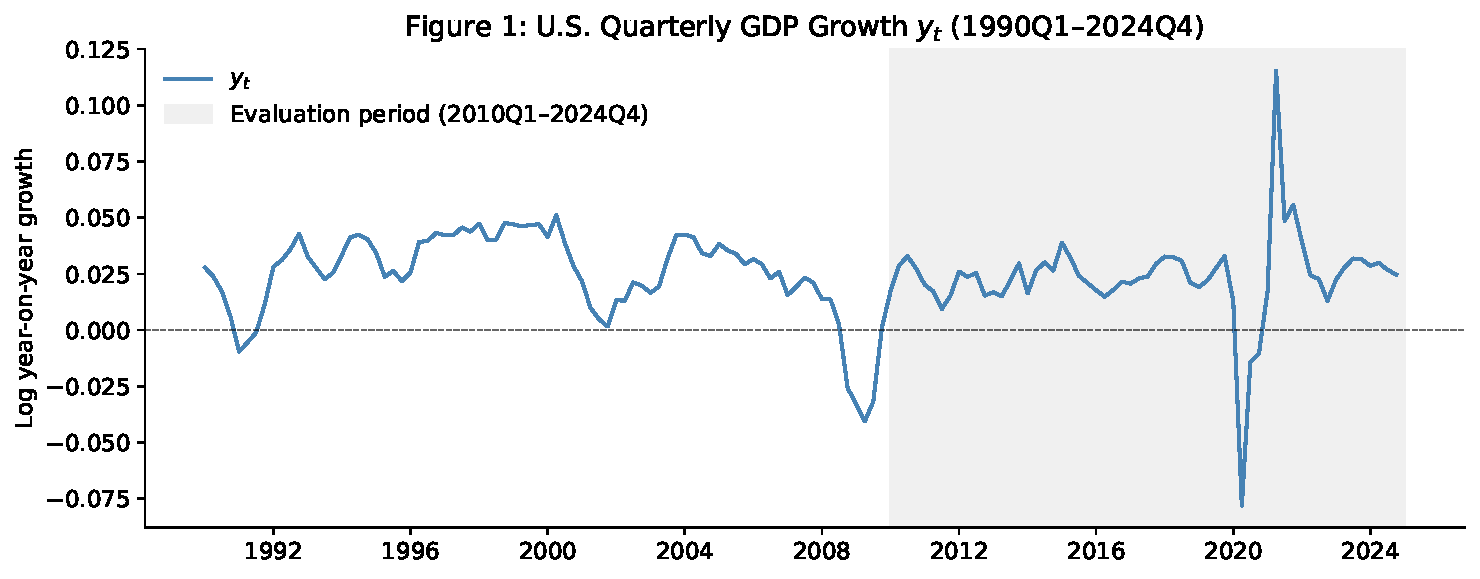
\includegraphics[width=\textwidth]{Assignment1/figures/fig1_gdp_growth.pdf}
    \caption{U.S. quarterly GDP growth $y_t$, 1990Q1--2024Q4.
             Shaded region indicates the out-of-sample evaluation period (2010Q1--2024Q4).}
    \label{fig:gdp_growth}
\end{figure}


% ─────────────────────────────────────────────────────────────────────────────
\section{Econometric Theory}\label{sec:p1-theory}
% ─────────────────────────────────────────────────────────────────────────────



We consider the ARMA($p$,$q$) model
\begin{equation}\label{eq:arma}
  y_t = \delta + \phi_1 y_{t-1} + \cdots + \phi_p y_{t-p}
        + \varepsilon_t + \theta_1 \varepsilon_{t-1} + \cdots + \theta_q \varepsilon_{t-q},
  \quad \varepsilon_t \overset{\text{i.i.d.}}{\sim} N(0,\sigma^2),
\end{equation}
where $y_t$ is the log year-on-year GDP growth rate and $\delta$ is the intercept; a pure AR($p$) corresponds to $q=0$. Writing $\phi(L) = 1 - \phi_1 L - \cdots - \phi_p L^p$, the process is stationary and weakly dependent iff all roots $z_j$ of $\phi(z)=0$ satisfy $|z_j|>1$ (equivalently, all inverse roots lie inside the unit circle). For $p=2$ this reduces to the triangle $\phi_1+\phi_2<1$, $\phi_2-\phi_1<1$, $|\phi_2|<1$. Under stationarity, $y_t$ admits an MA($\infty$) representation with unconditional mean $\mu = \delta/(1 - \phi_1 - \cdots - \phi_p)$.

\subsection{Estimation}

For AR($p$) models, parameters are estimated by OLS, which under $\varepsilon_t\sim N(0,\sigma^2)$ coincides with MLE. Under stationarity, weak dependence, and $E[\varepsilon_t\mid\mathcal{I}_{t-1}]=0$, $\hat{\boldsymbol{\phi}}$ is consistent and asymptotically normal, so a single coefficient is tested by the Wald $t$-ratio $H_0\colon \phi_j=0,\ t_{\phi_j} = \hat\phi_j/\widehat{\mathrm{s.e.}}(\hat\phi_j)\xrightarrow{d} N(0,1)$.
\newline
For ARMA($p$,$q$) with $q\geq 1$, OLS is infeasible (lagged $\varepsilon_t$ are unobserved); we estimate by Gaussian MLE with the conditional log-likelihood (given $y_1,\ldots,y_p$)
$$
\ell(\boldsymbol{\phi},\boldsymbol{\theta},\sigma^2)= -\tfrac{T}{2}\log(2\pi\sigma^2)-\tfrac{1}{2\sigma^2}\sum_{t=1}^{T}\varepsilon_t^2,
$$
where residuals are computed recursively.
\newline
Model selection follows a general-to-specific (GETS) strategy: starting from AR(4), nested restrictions are tested by the likelihood-ratio statistic
$$
\xi_{\mathrm{LR}}=-2\bigl(\log L(\tilde{\boldsymbol{\theta}})-\log L(\hat{\boldsymbol{\theta}})\bigr)\xrightarrow{d}\chi^2(j)
$$
for $j$ restrictions. Because LR is sensitive to non-normality (and invalid under QMLE), each reduction is cross-checked with AIC and BIC; we use BIC as the primary criterion for its stronger complexity penalty.


\subsection{Forecasting}

The one-step-ahead forecast from~(\ref{eq:arma}) is $\hat{y}_{t+1}=E[y_{t+1}\mid\mathcal{I}_t]$, with parameters fixed at their training-sample estimates and residuals updated recursively via $\hat{\varepsilon}_t = y_t - \hat{y}_t$ for $t>T$. Forecasts are compared to the naive benchmark $\bar{y} = T^{-1}\sum_{t=1}^{T} y_t$ by RMSE and the Diebold--Mariano (DM) test on the squared-error differential $d_t = e_{\mathrm{model},t}^2 - e_{\mathrm{naive},t}^2$: under $H_0\colon E[d_t]=0$, $t_{\mathrm{DM}} = \bar{d}/\widehat{\mathrm{s.e.}}(\bar{d}) \xrightarrow{d} N(0,1)$, with $\widehat{\mathrm{s.e.}}(\bar{d})$ a HAC estimator (autocorrelated $d_t$).

\subsection{Growth-at-Risk}

The one-period Growth-at-Risk at risk level $\alpha\in(0,1)$ is the $\alpha$-quantile of $y_t\mid\mathcal{I}_{t-1}$: $P(y_t \leq \mathrm{GaR}^\alpha_t \mid \mathcal{I}_{t-1}) = \alpha$. Under $\varepsilon_t \sim N(0,\sigma^2)$,
\begin{equation}\label{eq:gar}
  \mathrm{GaR}^\alpha_t = \hat{y}_t + \sigma\Phi^{-1}(\alpha),
\end{equation}
where $\Phi^{-1}(\alpha)$ is the standard-normal $\alpha$-quantile.
\newline
Evaluation uses the hit indicator $\mathrm{hit}_t = \mathbf{1}\{y_t < \mathrm{GaR}^\alpha_t\}$ and violation rate $\hat{p} = T^{-1}\sum_t \mathrm{hit}_t$; under correct specification $(\mathrm{hit}_t)$ is i.i.d.\ Bernoulli($\alpha$), and $H_0\colon E[\mathrm{hit}_t]=\alpha$ is tested by $t = (\hat{p}-\alpha)/\sqrt{\alpha(1-\alpha)/T} \xrightarrow{d} N(0,1)$. Magnitudes are captured by the tick loss $\mathcal{T}_\alpha(y_t, \mathrm{GaR}^\alpha_t) = (\alpha - \mathrm{hit}_t)(y_t - \mathrm{GaR}^\alpha_t)$.


% ─────────────────────────────────────────────────────────────────────────────
\section{Empirical Analysis}\label{sec:p1-empirical}
% ─────────────────────────────────────────────────────────────────────────────

\subsection{Model Selection}

Figure~\ref{fig:acf_pacf} motivated a focus on AR models: the PACF is statistically significant at lags 1 and 2 and negligible thereafter. Following the GETS principle, we estimate AR(1)--AR(4) and ARMA(1,1) and compare them in Table~\ref{tab:model_selection}, then apply sequential LR tests starting from AR(4) to justify reducing the model.
\newline
\newline
Testing AR(4) vs.\ AR(3) ($H_0\colon \phi_4=0$) gives $\xi_{\mathrm{LR}}=0.08$ ($p=0.78$): fail to reject, reduce. Testing AR(3) vs.\ AR(2) ($H_0\colon \phi_3=0$) gives $\xi_{\mathrm{LR}}=2.29$ ($p=0.13$): again fail to reject, yielding AR(2) as the GETS outcome. Information criteria confirm: AR(2) achieves the best BIC ($-542.33$), while AR(1) is excluded due to significant residual autocorrelation ($Q(8)$, $p=0.00$, see Table~\ref{tab:model_selection}). We therefore select \textbf{AR(2)} as the preferred specification.

\begin{figure}[H]
    \centering
    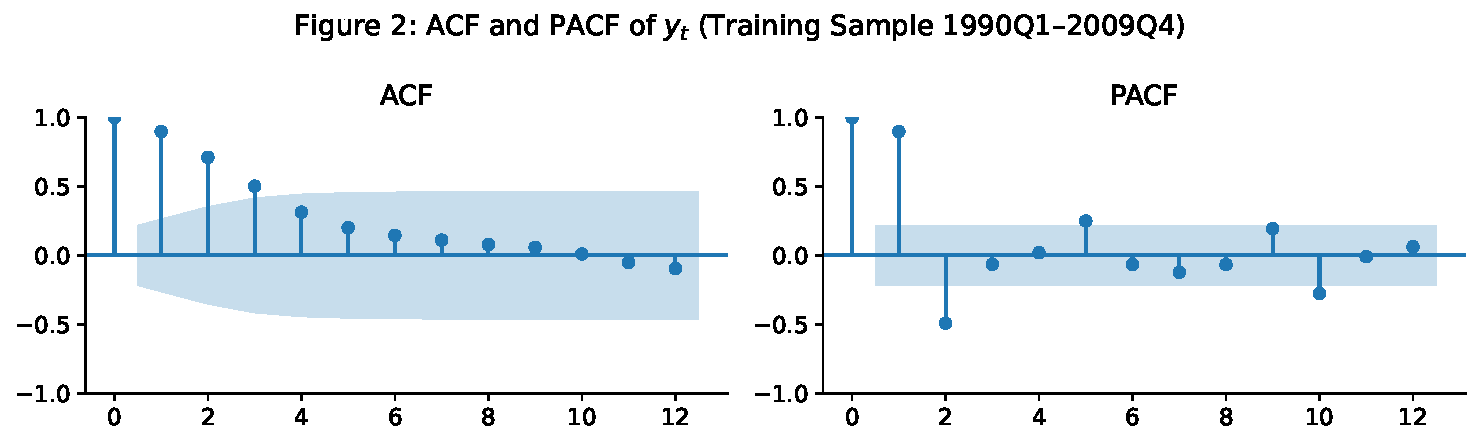
\includegraphics[width=\textwidth]{Assignment1/figures/fig2_acf_pacf.pdf}
    \caption{Sample ACF and PACF of $y_t$, training sample 1990Q1--2009Q4.
             Shaded regions indicate the $\pm 1.96/\sqrt{T}$ 95\% confidence bands.}
    \label{fig:acf_pacf}
\end{figure}

\begin{table}[H]
  \centering
  \caption{Model comparison: AIC, BIC, $\hat{{\sigma}}$, and Ljung-Box p-value (training sample 1990Q1--2009Q4).}
  \label{tab:model_selection}
  \begin{tabular}{lrrrr}
  \toprule
  Model & AIC & BIC & σ̂ & LB p-val (lag 8) \\
  \midrule
  AR(1) & -535.78 & -528.64 & 0.01 & 0.00 \\
  AR(2) & -551.86 & -542.33 & 0.01 & 0.14 \\
  AR(3) & -552.15 & -540.24 & 0.01 & 0.24 \\
  AR(4) & -550.23 & -535.94 & 0.01 & 0.28 \\
  ARMA(1,1) & -546.13 & -536.60 & 0.01 & 0.12 \\
  \bottomrule
  \end{tabular}
\end{table}



\subsection{Misspecification Testing}

Three misspecification tests are applied to the AR(2) training-sample residuals.
\newline
The Ljung-Box test (adjusted for $p=2$ AR parameters, $\sim\chi^2(h-p)$) yields $Q(4)=8.67$ ($p=0.013$) and $Q(8)=12.25$ ($p=0.057$). The borderline rejections are attributable to the 2008Q4 GFC outlier inflating nearby autocorrelations, not to a failure of the AR(2) lag structure.
\newline
\newline
The Jarque-Bera test yields $\mathrm{JB}=8.63$ ($p=0.013$), rejecting normality due to excess kurtosis of $1.31$ from GFC residuals in 2008Q4--2009Q1; adding intervention dummies for these quarters reduces it to $\mathrm{JB}=0.26$ ($p=0.879$), confirming the rejection is outlier-driven. We retain the plain AR(2), so the estimator is formally a QMLE: $t$-statistics remain valid under the sandwich covariance $\Omega^*=\mathcal{I}^{-1}\mathcal{J}\mathcal{I}^{-1}$, but the Gaussian GaR~(\ref{eq:gar}) may mis-calibrate the lower tail.
\newline
The ARCH-LM test at four lags yields $7.98$ ($p=0.092$), failing to reject conditional homoskedasticity at the 5\% level.

\subsection{Preferred Model: Estimates and Interpretation}

Table~\ref{tab:estimates} reports the ML estimates for the AR(2) model over 1990Q1--2009Q4. The estimated unconditional mean is $\hat{\mu} = 0.0262$ (standard error $0.006$), corresponding to an average annual GDP growth of approximately 2.6\%, which is in line with the U.S.\ long-run average. Both AR coefficients are highly significant: $\hat{\phi}_1 = 1.359$ ($t=11.0$) and $\hat{\phi}_2 = -0.512$ ($t=-4.1$). All three AR(2) triangle conditions hold ($\hat\phi_1+\hat\phi_2=0.847<1$, $\hat\phi_2-\hat\phi_1=-1.871<1$, $|\hat\phi_2|=0.512<1$), so the process is stationary; the inverse roots are complex conjugates with modulus $\approx 0.72$, implying damped oscillations around the mean. The residual standard deviation $\hat{\sigma}=0.010$ enters the GaR formula as the scale of the conditional distribution.

\begin{table}[H]
  \centering
  \caption{Estimation results for the AR(2) model (training sample 1990Q1--2009Q4).}
  \label{tab:estimates}
  \begin{tabular}{lrrrr}
  \toprule
   & Coefficient & Std. Error & t-stat & p-value \\
  \midrule
  const & 0.0262 & 0.0060 & 4.3455 & 0.0000 \\
  ar.L1 & 1.3587 & 0.1235 & 11.0055 & 0.0000 \\
  ar.L2 & -0.5118 & 0.1241 & -4.1237 & 0.0000 \\
  sigma2 & 0.0001 & 0.0000 & 6.5740 & 0.0000 \\
  \bottomrule
  \end{tabular}
\end{table}



\subsection{Forecast Evaluation}

Figure~\ref{fig:forecasts} and Table~\ref{tab:forecast_eval} present the out-of-sample results. The AR(2) RMSE is $0.0256$ versus $0.0206$ for the naive benchmark. The Diebold-Mariano statistic $t_{\mathrm{DM}}=1.186$ ($p=0.236$, HAC) fails to reject equal MSE; the gap is driven primarily by the COVID-19 shock, which lies outside the dynamics of any linear AR model.

\begin{figure}[H]
    \centering
    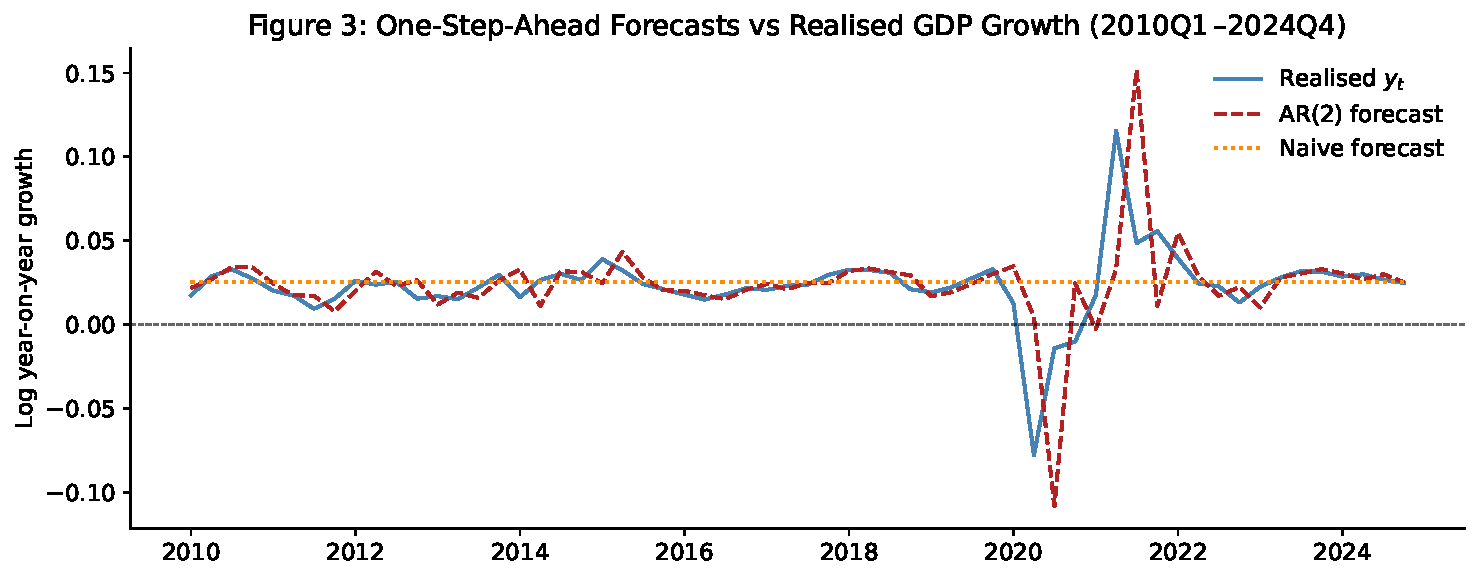
\includegraphics[width=0.8\textwidth]{Assignment1/figures/fig3_forecasts.pdf}
    \caption{Out-of-sample forecasts vs realised GDP growth, 2010Q1--2024Q4.}
    \label{fig:forecasts}
\end{figure}

\begin{table}[H]
  \centering
  \caption{Forecast evaluation: RMSE and Diebold-Mariano test (2010Q1--2024Q4).}
  \label{tab:forecast_eval}
  \begin{tabular}{lrrr}
  \toprule
  Model & RMSE & DM statistic & DM p-value \\
  \midrule
  AR(2) & 0.0256 & 1.0450 & 0.2960 \\
  Naive & 0.0206 & — & — \\
  \bottomrule
  \end{tabular}
\end{table}



\subsection{Growth-at-Risk Evaluation}

Figure~\ref{fig:gar} and Table~\ref{tab:gar_eval} present the GaR evaluation.
\newline
The AR(2) GaR has a violation rate of $\hat{p}=0.150$; the coverage $t$-test ($t=1.291$, $p=0.197$) cannot reject correct coverage. The $\mathrm{GaR}^{\mathrm{np}}$ series shows the mirror pattern ($\hat{p}=0.050$, same $|t|$, $p=0.197$), also not rejected. The AR(2) excess violations are largely attributable to the two COVID-19 quarters of 2020. On tick loss, $\mathrm{GaR}^{\mathrm{np}}$ achieves a marginally lower mean loss ($0.0040$ vs.\ $0.0046$). Mechanically, excess kurtosis (cf.\ JB in \S4.2) pushes the true 10\%-quantile below $\hat{y}_t+\hat\sigma\Phi^{-1}(0.10)$, so Gaussian GaR understates risk in turbulent quarters such as 2020. Overall, the AR(2) GaR provides useful time-variation relative to the constant benchmark but does not achieve demonstrably better calibration over this evaluation window.

\begin{figure}[H]
    \centering
    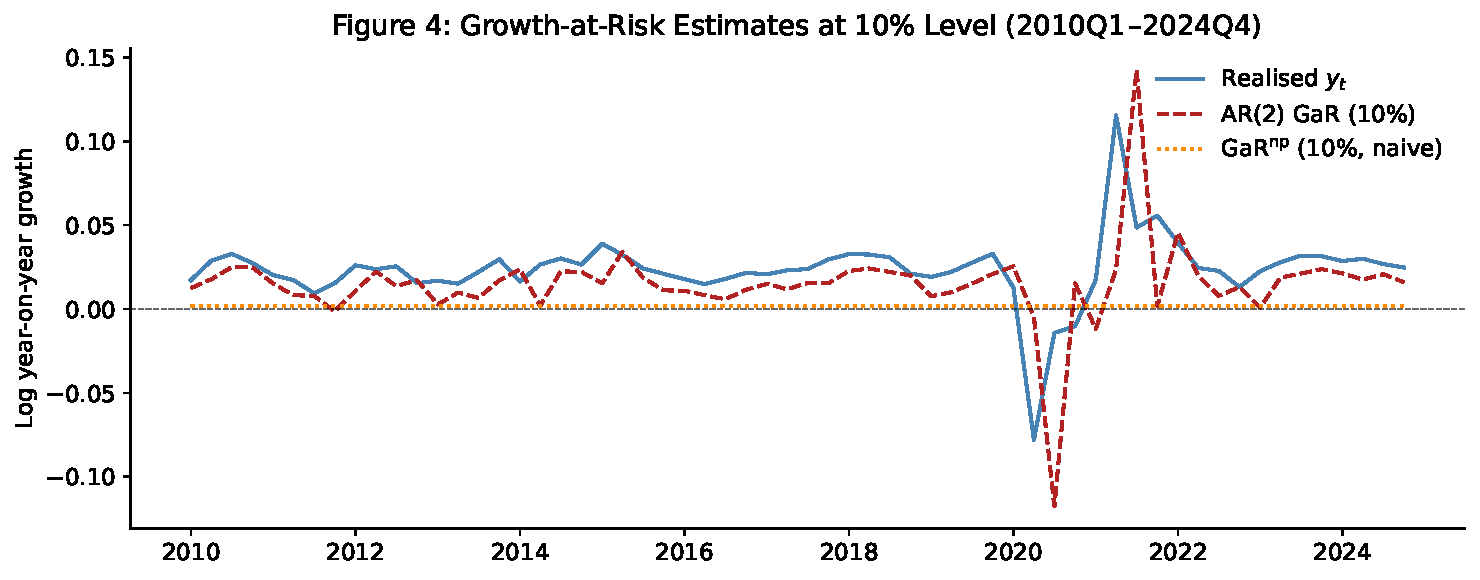
\includegraphics[width=0.8\textwidth]{Assignment1/figures/fig4_gar.pdf}
    \caption{Growth-at-Risk estimates (10\% level) vs realised GDP growth, 2010Q1--2024Q4.}
    \label{fig:gar}
\end{figure}

\begin{table}[H]
  \centering
  \caption{GaR evaluation at 10\% level: violation rates, coverage test, and tick loss (2010Q1--2024Q4).}
  \label{tab:gar_eval}
  \begin{tabular}{lrrrr}
  \toprule
  GaR series & Violation rate p̂ & t-stat (H₀: p̂ = 0.10) & p-value & Mean tick loss \\
  \midrule
  AR(2) GaR & 0.1500 & 1.2910 & 0.1970 & 0.0046 \\
  GaR_np (naive) & 0.0500 & -1.2910 & 0.1970 & 0.0040 \\
  \bottomrule
  \end{tabular}
\end{table}




% ─────────────────────────────────────────────────────────────────────────────
\section{Discussion}\label{sec:p1-discussion}
% ─────────────────────────────────────────────────────────────────────────────

Three limitations deserve mention.
First, the Gaussian derivation of~(\ref{eq:gar}) is contradicted by the JB rejection (\S4.2), so the non-rejection of the 10\% coverage test should be read as weak evidence of calibration, not validation of the full conditional distribution.
\newline
Second, parameters are estimated once on 1990Q1--2009Q4 and held fixed, ruling out coefficient drift, level shifts, and changing shock volatility during the evaluation window; the univariate specification additionally ignores macro-financial state variables that may carry incremental information about downside risk.
\newline
Third, the evaluation window is short and dominated by rare extremes: the COVID-19 collapse and rebound drive a disproportionate share of squared errors and GaR exceedances, so the headline metrics are sensitive to a handful of quarters and the conclusions are best read as evidence of robustness through an unusually turbulent sample rather than a universal performance statement.




% ─────────────────────────────────────────────────────────────────────────────
\section{Conclusion}\label{sec:p1-conclusion}
% ─────────────────────────────────────────────────────────────────────────────

An AR(2) for U.S.\ quarterly GDP growth was selected by GETS and confirmed by BIC, with misspecification tests passing at the 5\% level (JB rejection outlier-driven; $t$-statistics valid under QMLE). Out-of-sample, forecasts are indistinguishable from the naive benchmark (DM $p=0.24$) and both GaR series pass the 10\% coverage test; the dominant driver of deviations is the COVID-19 shock, consistent with simple univariate models remaining competitive in macroeconomic forecasting and risk quantification.

\bigskip
\noindent\textbf{References}

\noindent Adrian, T., N. Boyarchenko, and D. Giannone (2019). Vulnerable Growth. \textit{American Economic Review}, 109(4), 1263--1289.

\noindent Adrian, T., H. Chen, M.-S. Dovi, and J.H. Lee (2025). Machine-learning Growth-at-Risk. \textit{arXiv:2506.00572}.


% ═══════════════════════════════════════════════════════════════════════════════
% PART 2 — A Dynamic Model for U.S. House Prices
% ═══════════════════════════════════════════════════════════════════════════════
\newpage
\part{Part 2 --- A Dynamic Model for U.S. House Prices}
\setcounter{section}{0}
\setcounter{figure}{0}
\setcounter{table}{0}
\setcounter{equation}{0}
\renewcommand{\thefigure}{2.\arabic{figure}}
\renewcommand{\thetable}{2.\arabic{table}}
\renewcommand{\theequation}{2.\arabic{equation}}

% ─────────────────────────────────────────────────────────────────────────────
\section{Introduction}\label{sec:p2-intro}
% ─────────────────────────────────────────────────────────────────────────────

Housing is the largest asset on the balance sheet of most U.S.\ households and house-price swings have, historically, propagated to the wider macro\-economy; the user-cost framework predicts that, in equilibrium, prices are tied to rents and to the mortgage rate. This report tests that prediction by estimating the long-run relation
\begin{equation}
    h_t = \alpha + \beta_1 r_t + \beta_2 m_t,
\end{equation}
where $h_t$ is log house prices, $r_t$ is log rent, and $m_t$ is the 30-year fixed mortgage rate. Using monthly data for 2012M1--2023M12, we estimate a CVAR with $k=4$ lags and an unrestricted constant by Gaussian maximum likelihood, test the strict user-cost restriction $\beta_1=1$ by a Johansen LR test, and check the sensitivity of the conclusion to extending the sample back to 2000M1.
\newline
\newline
We find one co-integrating relation, but a rent elasticity statistically above one and a mortgage coefficient indistinguishable from zero, so the strict user-cost benchmark is rejected; equilibrium adjustment is borne almost entirely by the mortgage rate, and the finding is sensitive to the inclusion of the 2008-09 crisis years.
% ─────────────────────────────────────────────────────────────────────────────
\section{Description of the Data}\label{sec:p2-data}
% ─────────────────────────────────────────────────────────────────────────────

The data come from \texttt{Assignment\_3.xlsx} and are based on FRED series for the S\&P/Case-Shiller U.S.
National Home Price Index, the CPI for rent of primary residence, and the 30-year fixed mortgage rate. The transformed variables are $h_t = \log(\text{HousePrice})$, $r_t = \log(\text{Rent})$, and $m_t = \text{MortgageRate}$. The effective sample contains 144 monthly observations.
\newline
\newline
Figure~\ref{fig:series_panel} shows that both $h_t$ and $r_t$ trend upward, while $m_t$ is much more cyclical and rises sharply in 2022--2023. The visual pattern is consistent with non-stationary behaviour and motivates a co-integration analysis rather than a stationary VAR in levels. Table~\ref{tab:summary_stats} reports basic moments of the three series.

\begin{figure}[H]
	\centering
	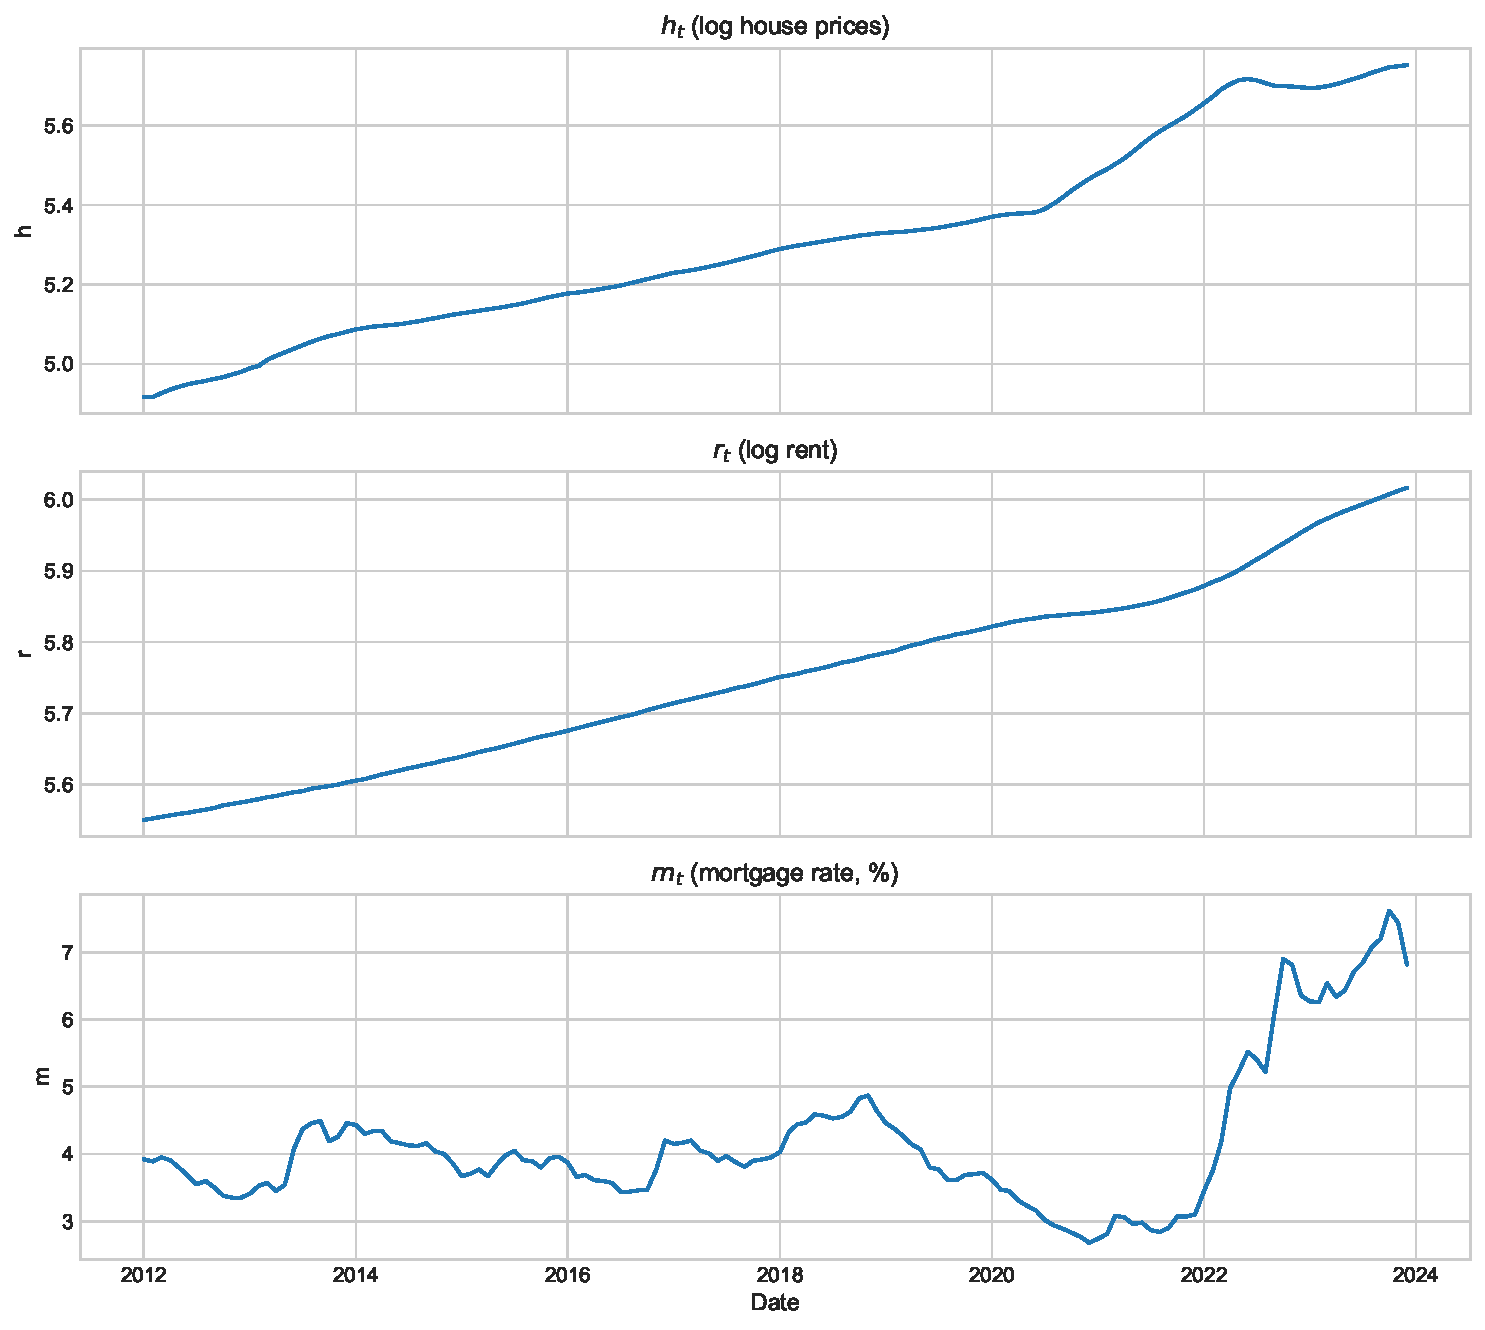
\includegraphics[width=0.7\textwidth]{Assignment3/figures/fig1_series_panel.pdf}
	\caption{Monthly series for $h_t$, $r_t$, and $m_t$, 2012M1--2023M12.}
	\label{fig:series_panel}
\end{figure}

\begin{table}[H]
\centering
\caption{Summary statistics for the analysis variables, 2012M1--2023M12.}
\label{tab:summary_stats}
\begin{tabular}{lrrrr}
\toprule
Variable & Mean & Std. Dev. & Min & Max \\
\midrule
h & 5.3108 & 0.2402 & 4.9165 & 5.7527 \\
r & 5.7511 & 0.1287 & 5.5501 & 6.0165 \\
m & 4.1642 & 1.0691 & 2.6800 & 7.6200 \\
\bottomrule
\end{tabular}
\end{table}


% ─────────────────────────────────────────────────────────────────────────────
\section{Econometric Theory}\label{sec:p2-theory}
% ─────────────────────────────────────────────────────────────────────────────

\paragraph{ADF testing.} For each variable $y_t$ we run an augmented Dickey--Fuller regression $\Delta y_t = (\rho-1) y_{t-1} + \sum_{j=1}^{p} \phi_j \Delta y_{t-j} + c + \varepsilon_t$ and test $H_0:\rho=1$ against $\rho<1$. The statistic is the $t$-ratio on $(\rho-1)$ and its asymptotic distribution is the non-standard Dickey--Fuller distribution (not $N(0,1)$); we use the constant-only critical values throughout. Lag length is selected by AIC.

\paragraph{The CVAR.} Let $X_t = (h_t, r_t, m_t)'$. Since the three series are treated as I(1), the natural framework is a co-integrated vector autoregression in error-correction form,
\begin{equation}
    \Delta X_t = \Pi X_{t-1} + \Gamma_1 \Delta X_{t-1} + \cdots + \Gamma_{k-1}\Delta X_{t-k+1} + \mu + e_t,
\end{equation}
where $\Pi$ contains long-run information, $\Gamma_j$ capture short-run dynamics, and $e_t$ is a zero-mean innovation. If $\Pi$ has reduced rank $r$, we can factorize $\Pi = \alpha\beta'$, so
\begin{equation}
    \Delta X_t = \alpha\beta'X_{t-1} + \Gamma_1 \Delta X_{t-1} + \cdots + \Gamma_{k-1}\Delta X_{t-k+1} + \mu + e_t.
    \label{eq:cvar}
\end{equation}
Here $\beta$ contains the co-integrating vectors and $\alpha_h, \alpha_r, \alpha_m$ measure how house prices, rents, and the mortgage rate respectively respond to disequilibrium in the long-run relation. The constant is unrestricted, so the long-run relation may include a non-zero intercept. We estimate \eqref{eq:cvar} by Gaussian maximum likelihood, which requires (i) correct lag length, (ii) i.i.d.\ Gaussian innovations, and (iii) constant parameters; rank inference is robust to non-normality, but inference on individual coefficients relies on the latter two assumptions.

\paragraph{Rank determination.} If $r=0$ there is no co-integration and the model reduces to a VAR in differences; if $0<r<p$ there are $r$ stationary long-run relations; if $r=p$ the system is stationary in levels. We test $H_0: \text{rank}(\Pi)\leq r_0$ against $H_1: \text{rank}(\Pi)>r_0$ by the Johansen trace statistic
\[
\mathrm{LR}_{\mathrm{trace}}(r_0) = -T\sum_{i=r_0+1}^{p}\ln(1-\hat{\lambda}_i),
\]
where $\hat\lambda_i$ are the ordered eigenvalues from the reduced-rank regression. The trace statistic has a non-standard asymptotic distribution depending on the deterministic specification; we use the case of an unrestricted constant in the VECM and the corresponding Johansen (1995) critical values. The procedure is sequential, starting at $r_0=0$ and stopping at the first non-rejection.

\paragraph{Restrictions on $\beta$.} A linear restriction of the form $\beta = H\phi$ (equivalently $R'\beta=0$ for $R=H_\perp$) is tested by the LR statistic
\[
\mathrm{LR} = -T\sum_{i=1}^{r}\!\left[\ln(1-\tilde\lambda_i)-\ln(1-\hat\lambda_i)\right]\;\stackrel{d}{\to}\;\chi^2(s),
\]
where $\tilde\lambda_i$ are the restricted eigenvalues and $s$ is the number of restrictions. We use this to test the strict user-cost restriction $\beta_r=1$, in which case $H=\bigl((1,-1,0)',(0,0,1)'\bigr)$ and $s=1$. Although $\hat\beta$ is super-consistent and mixed-Gaussian (while $\hat\alpha$ is $\sqrt{T}$-Gaussian), the LR statistic for smooth restrictions of this form is still asymptotically $\chi^2(s)$ under standard regularity. An analogous LR test of $\alpha = A\psi$ (a restriction on the loadings) has distribution $\chi^2(r\cdot(p-m))$, with $m=\dim(\psi)$; in particular, weak exogeneity of variable $i$ for $\beta$ corresponds to setting the $i$-th row of $\alpha$ to zero.

% ─────────────────────────────────────────────────────────────────────────────
\section{Empirical Analysis}\label{sec:p2-empirical}
% ─────────────────────────────────────────────────────────────────────────────

\subsection{Integration Properties}

Table~\ref{tab:unit_root_tests} reports ADF tests. The level series are clearly non-stationary: the null of a unit root is not rejected for $h_t$, $r_t$, or $m_t$. In first differences the null is rejected for $h_t$ and $m_t$ at the 5\% level, while $\Delta r_t$ is borderline ($p=0.087$), which is not unusual in a short monthly sample with strong persistence in rents. Taken together, the evidence is consistent with treating the three series as I(1) and proceeding to co-integration testing.

\begin{table}[H]
\centering
\caption{ADF unit-root tests (constant included).}
\label{tab:unit_root_tests}
\small
\setlength{\tabcolsep}{4pt}
\begin{tabular}{lrrr rrr}
\toprule
& \multicolumn{3}{c}{Level} & \multicolumn{3}{c}{First difference} \\
\cmidrule(lr){2-4}\cmidrule(lr){5-7}
Variable & Stat. & p-value & Lags & Stat. & p-value & Lags \\
\midrule
$h$ &  0.2679 & 0.9758 & 14 & -3.2160 & 0.0191 & 1 \\
$r$ &  1.7251 & 0.9982 & 12 & -2.6296 & 0.0870 & 8 \\
$m$ & -1.6255 & 0.4698 &  5 & -3.6555 & 0.0048 & 4 \\
\bottomrule
\end{tabular}
\normalsize
\end{table}


\subsection{Lag Selection}

Lag length is chosen by estimating a VAR in levels and minimising AIC; Table~\ref{tab:lag_selection} shows that AIC is minimised at lag 4, with BIC and HQIC also pointing to lag 4 within the displayed range. The preferred VECM therefore uses $k_{\Delta}=3$ lagged differences.

\begin{table}[H]
\centering
\caption{Lag-order selection criteria for VAR in levels (2012M1--2023M12).}
\label{tab:lag_selection}
\begin{tabular}{lrrr}
\toprule
Lag & AIC & BIC & HQIC \\
\midrule
0 & -10.3391 & -10.2736 & -10.3124 \\
1 & -29.0146 & -28.7525 & -28.9081 \\
2 & -30.7035 & -30.2449 & -30.5171 \\
3 & -30.9077 & -30.2525 & -30.6414 \\
4 & -31.1498 & -30.2980 & -30.8037 \\
5 & -31.1138 & -30.0655 & -30.6878 \\
6 & -31.0758 & -29.8309 & -30.5699 \\
7 & -31.0536 & -29.6122 & -30.4679 \\
8 & -31.0042 & -29.3662 & -30.3386 \\
9 & -31.0864 & -29.2519 & -30.3409 \\
10 & -31.0830 & -29.0519 & -30.2577 \\
11 & -31.0071 & -28.7795 & -30.1019 \\
12 & -30.9735 & -28.5494 & -29.9885 \\
\bottomrule
\end{tabular}
\end{table}


\subsection{Co-Integration Rank}

With the dynamic specification fixed, we test the co-integration rank. Table~\ref{tab:johansen_trace} reports the Johansen trace statistic at each $r_0$. For $H_0:r=0$ against $H_1:r\geq 1$, the statistic of $48.23$ exceeds the 5\% critical value of $29.80$, so we reject. For $H_0:r\leq 1$ against $H_1:r\geq 2$, the statistic of $11.56$ is below the 5\% critical value of $15.49$, so we do not reject. The preferred rank is therefore $r=1$.

\begin{table}[H]
\centering
\caption{Johansen trace test. Sequential procedure rejects if trace stat. exceeds the 5\% critical value.}
\label{tab:johansen_trace}
\begin{tabular}{lrrrr}
\toprule
$H_0$ & Trace stat. & CV 90\% & CV 95\% & CV 99\% \\
\midrule
$r=0$ & 48.2266 & 27.0669 & 29.7961 & 35.4628 \\
$r\leq 1$ & 11.5648 & 13.4294 & 15.4943 & 19.9349 \\
$r\leq 2$ & 3.6207 & 2.7055 & 3.8415 & 6.6349 \\
\bottomrule
\end{tabular}
\end{table}


Having found rank $r=1$, we estimate the CVAR and characterise the long-run relation. Figure~\ref{fig:coint_fit} plots the actual $h_t$ together with the fitted long-run component implied by the normalised co-integrating vector, and Table~\ref{tab:cvar_estimates} reports the implied coefficients with ML standard errors.

\begin{table}[H]
\centering
\caption{Preferred CVAR (k=4, unrestricted constant, rank 1). Normalised on $h_t$. Std. err.\ from VECM ML.}
\label{tab:cvar_estimates}
\begin{tabular}{lrr}
\toprule
Parameter & Estimate & Std. err. \\
\midrule
$\beta_r$ (rent elasticity) & 1.4918 & 0.0467 \\
$\beta_m$ (mortgage coef.) & 0.0085 & 0.0068 \\
$\alpha_h$ & 0.0156 & 0.0049 \\
$\alpha_r$ & 0.0091 & 0.0018 \\
$\alpha_m$ & 0.3958 & 0.5380 \\
\bottomrule
\end{tabular}
\end{table}


\begin{figure}[H]
	\centering
	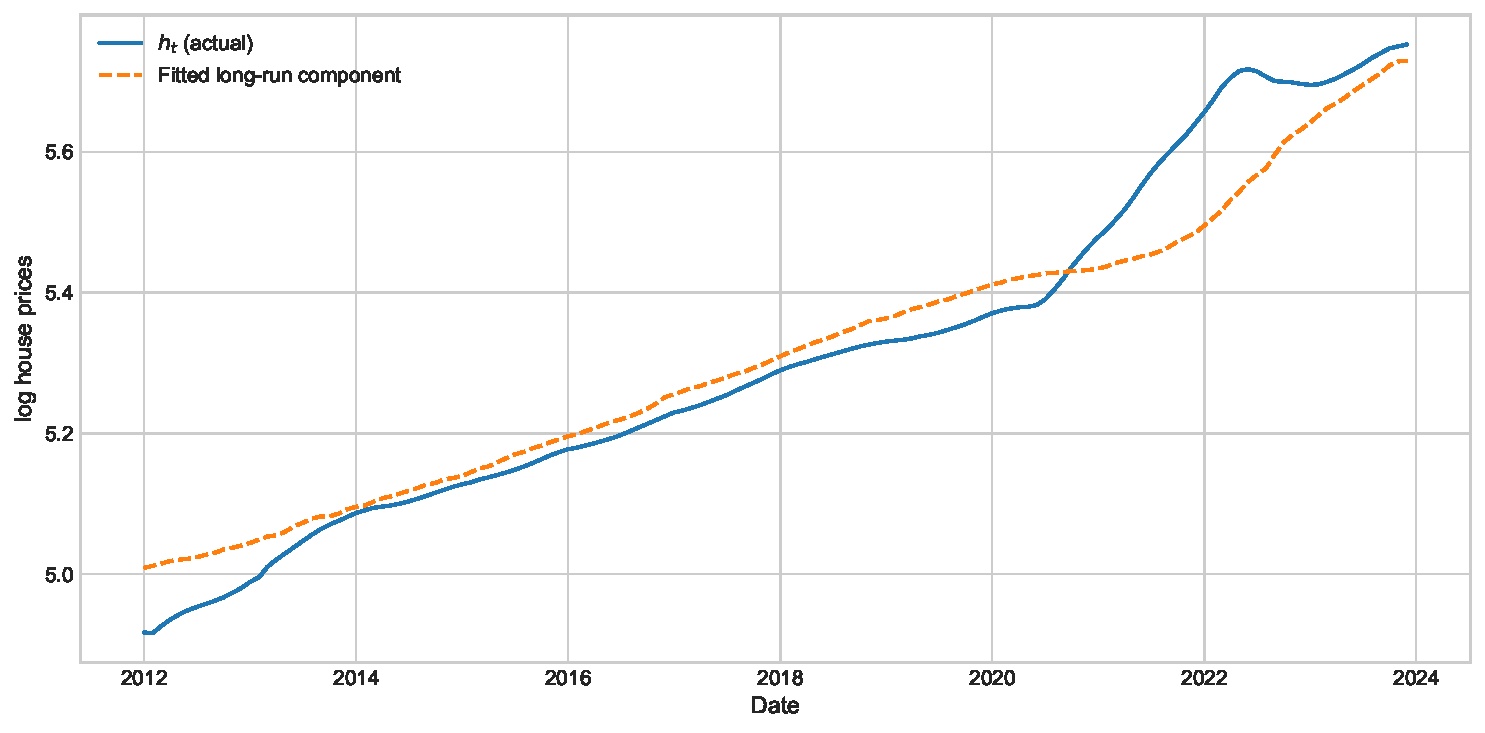
\includegraphics[width=0.9\textwidth]{Assignment3/figures/fig2_cointegration_fit.pdf}
	\caption{Actual $h_t$ and fitted long-run component from the preferred CVAR.}
	\label{fig:coint_fit}
\end{figure}

\subsection{Misspecification Diagnostics}

Before testing the user-cost restriction, we assess whether the dynamic specification is adequate. Residual diagnostics in Table~\ref{tab:diagnostics} are mixed. The Portmanteau whiteness test ($p=0.30$) finds no remaining serial correlation, so the dynamic specification is statistically adequate in that dimension. The Jarque--Bera test strongly rejects normality, and ARCH-LM rejects homoskedasticity for the mortgage-rate residuals at the 5\% level ($p=0.022$) and is borderline for $h_t$ ($p=0.086$). These results support consistency of the rank estimate (which does not rely on Gaussianity), but the violations of normality and homoskedasticity imply that the standard errors on $\beta$ and $\alpha$ should be read with caution and that asymptotic-normality based tests are at best approximate; the post-2021 interest-rate shock is the likely driver. The LR statistics reported below remain asymptotically $\chi^2$ under the maintained assumptions, but their finite-sample $p$-values should be treated as approximate.

\begin{table}[H]
\centering
\caption{Misspecification diagnostics for the preferred CVAR specification.}
\label{tab:diagnostics}
\begin{tabular}{lrr}
\toprule
Test & Statistic & p-value \\
\midrule
Whiteness (Portmanteau) & 83.9923 & 0.3012 \\
Normality (Jarque--Bera) & 391.7401 & 0.0000 \\
ARCH LM (h) & 19.1037 & 0.0861 \\
ARCH LM (r) & 6.4636 & 0.8909 \\
ARCH LM (m) & 23.7053 & 0.0223 \\
\bottomrule
\end{tabular}
\end{table}


\subsection{Preferred CVAR and the User-Cost Restriction}

Normalising on house prices, the estimated long-run relation is
\begin{equation}
	h_t = \hat c + 1.4918\,r_t + 0.0085\,m_t,
\end{equation}
with ML standard errors of $0.0467$ on the rent coefficient and $0.0068$ on the mortgage-rate coefficient. The rent elasticity is statistically and economically larger than one (a $z$-ratio of $(1.4918-1)/0.0467 \approx 10.5$ rejects $\beta_r=1$ at any conventional level), and the mortgage coefficient is small, statistically insignificant ($t\approx 1.25$), and has the wrong sign relative to the user-cost prediction $\beta_2<0$. The formal Johansen LR test of the strict user-cost restriction $\beta_r=1$ in Table~\ref{tab:restriction_test} corroborates this: the LR statistic of $14.46$ has a $\chi^2(1)$ $p$-value of $0.0001$, so we strongly reject unit rent elasticity. The data support a stable long-run link between house prices, rents, and the mortgage rate, but they reject the exact sign and magnitude pattern of the textbook model.

The adjustment loadings indicate how equilibrium is restored. The point estimate $\hat\alpha_m=0.3958$ looks large but has standard error $0.5380$, so a $t$-ratio of $0.74$ means we cannot distinguish $\alpha_m$ from zero; the mortgage equation's apparent correction is not statistically supported. The loadings $\hat\alpha_h=0.0156$ ($t\approx 3.2$) and $\hat\alpha_r=0.0091$ ($t\approx 5.0$) are statistically significant but economically tiny. To make this precise we formally test weak exogeneity of the mortgage rate for $\beta$, i.e.\ the restriction $\alpha_m=0$, using the Johansen LR procedure on $\alpha = A\psi$ with $A=\bigl((1,0,0)',(0,1,0)'\bigr)$. Table~\ref{tab:restriction_test} reports an LR statistic of $0.45$ with $\chi^2(1)$ $p$-value $0.50$, so we do not reject weak exogeneity of $m_t$. The economic picture is therefore that short-run correction is borne by the two slow-moving prices ($h_t$ and $r_t$), with the mortgage rate behaving as the (weakly) exogenous driver of the system --- which is again the opposite of the user-cost story, in which house prices adjust to the rent--cost wedge.

\begin{table}[H]
\centering
\caption{Johansen LR test of the strict user-cost restriction $\beta_r=1$. $H_0$: unit rent elasticity; asymptotic distribution $\chi^2(1)$.}
\label{tab:restriction_test}
\begin{tabular}{lrrr}
\toprule
Test & Statistic & d.f. & p-value \\
\midrule
LR test $\beta_r = 1$ & 14.4616 & 1 & 0.0001 \\
\bottomrule
\end{tabular}
\end{table}


% ─────────────────────────────────────────────────────────────────────────────
\section{Discussion}\label{sec:p2-discussion}

The empirical evidence supports one co-integrating relation between house prices, rents, and the mortgage rate in 2012M1--2023M12, but the economic content of the relation is only partly aligned with the textbook user-cost model: the rent elasticity is significantly above one, the mortgage-rate coefficient has the wrong sign and is insignificant, and the formal LR test of $\beta_r=1$ is rejected at $p=0.0001$. Simpler frictions absent from \eqref{eq:cvar} --- risk premia, refinancing constraints, supply rigidities, expectational shifts --- offer natural explanations for the elasticity exceeding one. Equilibrium is also restored in a way that the textbook does not predict: the mortgage rate, not house prices, does most of the short-run adjusting toward the long-run wedge.

\begin{table}[H]
\centering
\caption{Robustness of the main results to extending the sample to 2000M1--2023M12.}
\label{tab:robustness}
\begin{tabular}{lrr}
\toprule
Quantity & 2012M1--2023M12 & 2000M1--2023M12 \\
\midrule
VAR lag (AIC) & 4 & 4 \\
Trace stat. at $r=0$ & 48.23 & 19.64 \\
Trace stat. at $r\leq 1$ & 11.56 & 3.68 \\
$\beta_r$ & 1.4918 & 1.5521 \\
$\beta_m$ & 0.0085 & 0.1719 \\
LR stat. ($\beta_r=1$) & 14.4616 & 2.7022 \\
LR $p$-value & 0.0001 & 0.1002 \\
\bottomrule
\end{tabular}
\end{table}


To gauge robustness we re-estimate the same specification on the longer sample 2000M1--2023M12, which includes the housing boom and the financial crisis. AIC again selects four lags, and the implied long-run coefficients ($\hat\beta_r=1.55$, $\hat\beta_m=0.17$) are qualitatively similar. The trace statistic at $r=0$ collapses to $19.6$, however --- below the 5\% critical value of $29.8$ --- so we cannot even reject no co-integration on the longer sample, and the LR test of $\beta_r=1$ has $p=0.10$, no longer significant at the 5\% level. The 2012--2023 finding is therefore sample-specific: the bubble--bust period is informative enough about the data-generating process that the post-crisis ``stable equilibrium'' interpretation does not survive its inclusion. This sensitivity, combined with the residual diagnostics, suggests the estimated long-run relation should be read as a useful approximation for the post-crisis regime rather than a structural law.

% ─────────────────────────────────────────────────────────────────────────────
\section{Conclusion}\label{sec:p2-conclusion}
% ─────────────────────────────────────────────────────────────────────────────

For 2012M1--2023M12 a CVAR with $k=4$ lags identifies one co-integrating relation among house prices, rents, and the mortgage rate. The strict user-cost benchmark is rejected: $\hat\beta_r=1.49$ with $p<10^{-4}$ for $H_0:\beta_r=1$, and the mortgage-rate coefficient is small, insignificant, and of the wrong sign. Equilibrium is restored mainly through the mortgage-rate equation, and the finding does not survive extension of the sample to include the 2000s boom and the 2008-09 crisis.

\bigskip
\noindent\textbf{References}

\noindent Anundsen, A.K. (2019). Detecting Imbalances in House Prices: What Goes Up Must Come Down? \textit{The Scandinavian Journal of Economics}, 121(4), 1587--1619.

\noindent Johansen, S. (1995). \textit{Likelihood-Based Inference in Cointegrated Vector Autoregressive Models}. Oxford University Press.


% ═══════════════════════════════════════════════════════════════════════════════
% PART 3 — The Additional Assignment
% ═══════════════════════════════════════════════════════════════════════════════
\newpage
\part{Part 3 --- The Additional Assignment}
\setcounter{section}{0}
\setcounter{figure}{0}
\setcounter{table}{0}
\setcounter{equation}{0}
\renewcommand{\thefigure}{3.\arabic{figure}}
\renewcommand{\thetable}{3.\arabic{table}}
\renewcommand{\theequation}{3.\arabic{equation}}

Throughout, we work with the VAR(1) model (5.1)--(5.3) and, for Questions~(3)--(7), the modified specification (5.5)--(5.7). The stationarity assumptions $|\phi_1|<1$ and $|\phi_3|<1$ are maintained.

% ─────────────────────────────────────────────────────────────────────────────
\subsection*{Question (1) -- Reduced-form impulse responses}\label{sec:p3-q1}
% ─────────────────────────────────────────────────────────────────────────────

\paragraph{(a) Closed form for $\phi_1\neq\phi_3$.} We show by induction on $k\geq 1$ that
\begin{equation}
\Phi^{k}=\begin{pmatrix} \phi_1^{k} & \phi_2\,\dfrac{\phi_1^{k}-\phi_3^{k}}{\phi_1-\phi_3} \\[4pt] 0 & \phi_3^{k}\end{pmatrix}. \label{eq:Phik}
\end{equation}

\textit{Base case $k=1$.} Directly, $\Phi^{(1)}_{12}=\phi_2=\phi_2(\phi_1-\phi_3)/(\phi_1-\phi_3)$, and the diagonal entries are $\phi_1,\phi_3$, as required.

\textit{Inductive step.} Assume \eqref{eq:Phik} holds for some $k\geq 1$. Because $\Phi$ is upper-triangular the product $\Phi^{k+1}=\Phi\,\Phi^{k}$ remains upper-triangular with diagonal $(\phi_1^{k+1},\phi_3^{k+1})$, and the $(1,2)$-element is
\begin{align*}
\Phi^{(k+1)}_{12} &= \phi_1\cdot\Phi^{(k)}_{12} + \phi_2\cdot\Phi^{(k)}_{22}
= \phi_1\,\phi_2\,\frac{\phi_1^{k}-\phi_3^{k}}{\phi_1-\phi_3} + \phi_2\,\phi_3^{k}\\
&= \frac{\phi_2}{\phi_1-\phi_3}\Big(\phi_1^{k+1}-\phi_1\phi_3^{k}+(\phi_1-\phi_3)\phi_3^{k}\Big)
= \phi_2\,\frac{\phi_1^{k+1}-\phi_3^{k+1}}{\phi_1-\phi_3}.
\end{align*}
This completes the induction and establishes (5.4).

\paragraph{(b) Special case $\phi_1=\phi_3$.} When the two diagonal entries coincide the geometric-difference quotient in \eqref{eq:Phik} is of indeterminate form $0/0$. Treating $\phi_3$ as the variable and applying L'H\^{o}pital's rule,
\begin{equation*}
\lim_{\phi_3\to\phi_1}\,\frac{\phi_1^{k}-\phi_3^{k}}{\phi_1-\phi_3}
= \lim_{\phi_3\to\phi_1}\frac{-k\phi_3^{k-1}}{-1}
= k\,\phi_1^{k-1},
\end{equation*}
so that
\begin{equation}
\Phi^{(k)}_{12}\bigg|_{\phi_1=\phi_3} = \phi_2\,k\,\phi_1^{k-1},\qquad k\geq 1.\label{eq:Phik-equal}
\end{equation}
The same expression is obtained directly by induction: $\Phi^{(k+1)}_{12}=\phi_1\,\phi_2 k\phi_1^{k-1}+\phi_2\phi_1^{k}=\phi_2(k+1)\phi_1^{k}$.

\paragraph{(c) Cumulated impulse response, $\phi_1\neq\phi_3$.} Note $\Phi^{0}=I$, so $\Phi^{(0)}_{12}=0$. For $|\phi_1|<1$ and $|\phi_3|<1$ the two geometric series below converge, and
\begin{align*}
\sum_{k=0}^{\infty}\Phi^{(k)}_{12}
&= \sum_{k=1}^{\infty}\phi_2\,\frac{\phi_1^{k}-\phi_3^{k}}{\phi_1-\phi_3}
= \frac{\phi_2}{\phi_1-\phi_3}\Bigg(\sum_{k=1}^{\infty}\phi_1^{k}-\sum_{k=1}^{\infty}\phi_3^{k}\Bigg)\\
&= \frac{\phi_2}{\phi_1-\phi_3}\!\left(\frac{\phi_1}{1-\phi_1}-\frac{\phi_3}{1-\phi_3}\right)
= \frac{\phi_2}{\phi_1-\phi_3}\cdot\frac{\phi_1-\phi_3}{(1-\phi_1)(1-\phi_3)}.
\end{align*}
Hence
\begin{equation}
\sum_{k=0}^{\infty}\Phi^{(k)}_{12} = \frac{\phi_2}{(1-\phi_1)(1-\phi_3)}.\label{eq:cumIRF}
\end{equation}
\textit{Interpretation.} This is the $(1,2)$-element of $(I-\Phi)^{-1}=\sum_{k=0}^{\infty}\Phi^{k}$ (which converges since both eigenvalues of $\Phi$ lie strictly inside the unit circle), and it measures the long-run effect on $y$ of a unit innovation in $\varepsilon_{2,t}$.

% ─────────────────────────────────────────────────────────────────────────────
\subsection*{Question (2) -- OLS consistency under conditional heteroskedasticity}\label{sec:p3-q2}
% ─────────────────────────────────────────────────────────────────────────────

We now suppose $\varepsilon_t=H_t^{1/2}u_t$ with $u_t$ i.i.d., $\E[u_t]=0$, $\Var(u_t)=I_2$, and $H_t$ a positive-definite, $\Info_{t-1}$-measurable conditional covariance matrix. The process $\{\varepsilon_t\}$ is assumed stationary.

\paragraph{Claim.} The equation-by-equation OLS estimator of $\Phi$ is \emph{consistent}.

\paragraph{Argument.} Writing the VAR(1) compactly as $Z_t = \Phi Z_{t-1}+\varepsilon_t$, the OLS estimator (on the system, equivalent equation-by-equation since the regressors are identical across equations) satisfies
\begin{equation*}
\widehat{\Phi}_{\text{OLS}} - \Phi
= \Bigg(\frac{1}{T}\sum_{t=1}^{T} \varepsilon_t Z_{t-1}'\Bigg)\Bigg(\frac{1}{T}\sum_{t=1}^{T} Z_{t-1}Z_{t-1}'\Bigg)^{-1}.
\end{equation*}
Two conditions secure consistency:

\medskip
\textit{(i) Orthogonality.} Because $H_t^{1/2}\in\Info_{t-1}$ and $u_t$ is i.i.d.\ and independent of $\Info_{t-1}$,
\begin{equation*}
\E[\varepsilon_t\mid\Info_{t-1}] = H_t^{1/2}\,\E[u_t]=0,
\end{equation*}
so by the law of iterated expectations $\E[\varepsilon_t Z_{t-1}']=\E\!\big[Z_{t-1}'\E[\varepsilon_t\mid\Info_{t-1}]\big]=0$. The unconditional moment condition that drives OLS is therefore preserved.

\medskip
\textit{(ii) LLN/ergodic theorem.} Stationarity of $\{(Z_t,\varepsilon_t)\}$ together with weak dependence (inherited from $|\phi_1|<1$, $|\phi_3|<1$ and the i.i.d.\ structure of $u_t$) ensures
\begin{equation*}
\frac{1}{T}\sum_{t=1}^{T}Z_{t-1}Z_{t-1}'\xrightarrow{p}\E[Z_{t-1}Z_{t-1}'],\qquad
\frac{1}{T}\sum_{t=1}^{T}\varepsilon_t Z_{t-1}'\xrightarrow{p}0,
\end{equation*}
the first limit being positive definite (otherwise some linear combination of $Z_{t-1}$ would be degenerate, contradicting stationarity with non-zero innovation variance). The continuous mapping theorem then yields $\widehat{\Phi}_{\text{OLS}}\xrightarrow{p}\Phi$.

\paragraph{Caveats.} Although consistent, OLS is no longer efficient: the Gauss--Markov / MLE-equals-OLS argument relied on $\E[\varepsilon_t\varepsilon_t'\mid\Info_{t-1}]=\Sigma$ being constant, which now fails. Two practical implications: (1) standard errors must be made heteroskedasticity-consistent (sandwich/HCSE form), and (2) an estimator that models $H_t$ explicitly (e.g.\ multivariate GARCH-based quasi-MLE) is asymptotically more efficient.

% ─────────────────────────────────────────────────────────────────────────────
\subsection*{Question (3) -- Unconditional variance in the ARCH-X model}\label{sec:p3-q3}
% ─────────────────────────────────────────────────────────────────────────────

We work with the modified model (5.5)--(5.7). Assuming a stationary solution exists, $\E[\varepsilon_t^2]$ is constant in $t$. By the law of iterated expectations,
\begin{equation*}
\E[\varepsilon_t^2]
= \E\!\big[\E[\varepsilon_t^2\mid\Info_{t-1}]\big]
= \E[\sigma_t^2]
= \omega + \alpha\,\E[\varepsilon_{t-1}^2] + \gamma\,\E[x_{t-1}^2].
\end{equation*}
The process $\{x_t\}$ is a stationary Gaussian AR(1) with $|\phi_3|<1$, $\E[x_t]=0$, and
\begin{equation}
\E[x_t^2] = \frac{\sigma_\eta^2}{1-\phi_3^2}.\label{eq:Vx}
\end{equation}
Imposing stationarity $\E[\varepsilon_t^2]=\E[\varepsilon_{t-1}^2]$ and solving,
\begin{equation}
\E[\varepsilon_t^2] = \frac{\omega+\gamma\,\sigma_\eta^2/(1-\phi_3^2)}{1-\alpha},\label{eq:Veps}
\end{equation}
which is (5.8).

\paragraph{Conditions for \eqref{eq:Veps} to be well-defined and strictly positive.}
\begin{equation*}
\omega>0,\quad \alpha\geq 0,\quad \gamma\geq 0,\quad \sigma_\eta^2>0,\quad |\phi_3|<1,\quad \alpha<1.
\end{equation*}
Under these, the numerator of \eqref{eq:Veps} is the sum of two non-negative terms with $\omega>0$, hence strictly positive, and the denominator $1-\alpha$ is strictly positive. (The strict inequality $\alpha<1$ is what is actually needed; positivity of $\omega$ and of $\sigma_\eta^2$ ensures the variance is strictly positive even at the boundary $\gamma=0$.)

\paragraph{Comparison with standard ARCH(1).} Setting $\gamma=0$ reduces \eqref{eq:Veps} to the familiar ARCH(1) unconditional variance $\omega/(1-\alpha)$ (cf.\ \S2 of the ARCH lecture notes). The additional term $\gamma\sigma_\eta^2/[(1-\alpha)(1-\phi_3^2)]$ captures the contribution of the persistent exogenous regressor $x_{t-1}^2$ to the unconditional variance of $\varepsilon_t$: a more persistent $x_t$ (larger $\phi_3^2$) or a more variable $\eta_t$ (larger $\sigma_\eta^2$) inflates $\E[\varepsilon_t^2]$, and the effect is amplified by the ARCH feedback through the factor $1/(1-\alpha)$.

% ─────────────────────────────────────────────────────────────────────────────
\subsection*{Question (4) -- Conditional joint density and log-likelihood}\label{sec:p3-q4}
% ─────────────────────────────────────────────────────────────────────────────

\paragraph{Factorization.} Conditional on $\Info_{t-1}$, the quantities $\sigma_t^2=\omega+\alpha\varepsilon_{t-1}^2+\gamma x_{t-1}^2$ and $\phi_3 x_{t-1}$ are constants (deterministic functions of the conditioning information and $\psi$). Since $z_t$ and $\eta_t$ are mutually independent and independent of $\Info_{t-1}$, the pair $(y_t,x_t)=(\phi_1 y_{t-1}+\phi_2 x_{t-1}+\sigma_t z_t,\,\phi_3 x_{t-1}+\eta_t)$ is, given $\Info_{t-1}$, a function of two independent random variables. Hence
\begin{equation}
f(y_t,x_t\mid\Info_{t-1};\psi) = f(y_t\mid\Info_{t-1};\psi)\,f(x_t\mid\Info_{t-1};\psi).\label{eq:factor}
\end{equation}
With $z_t\sim N(0,1)$ and $\eta_t\sim N(0,\sigma_\eta^2)$,
\begin{align}
f(y_t\mid\Info_{t-1};\psi)
&= \frac{1}{\sqrt{2\pi\,\sigma_t^2}}\exp\!\left(-\frac{(y_t-\phi_1 y_{t-1}-\phi_2 x_{t-1})^2}{2\sigma_t^2}\right),\label{eq:fy}\\
f(x_t\mid\Info_{t-1};\psi)
&= \frac{1}{\sqrt{2\pi\,\sigma_\eta^2}}\exp\!\left(-\frac{(x_t-\phi_3 x_{t-1})^2}{2\sigma_\eta^2}\right).\label{eq:fx}
\end{align}

\paragraph{Log-likelihood.} Treating $(y_0,x_0,\varepsilon_0)$ as given initial conditions, the conditional log-likelihood for the sample $\{(y_t,x_t)\}_{t=1}^{T}$ is, by \eqref{eq:factor},
\begin{align}
\ell_T(\psi)
&= \sum_{t=1}^{T}\log f(y_t\mid\Info_{t-1};\psi) + \sum_{t=1}^{T}\log f(x_t\mid\Info_{t-1};\psi)\nonumber\\
&\equiv \ell_T^{y}(\theta_y) + \ell_T^{x}(\theta_x),\label{eq:ll-split}
\end{align}
where $\theta_y=(\phi_1,\phi_2,\omega,\alpha,\gamma)'$ and $\theta_x=(\phi_3,\sigma_\eta^2)'$, with
\begin{align}
\ell_T^{y}(\theta_y) &= -\frac{T}{2}\log(2\pi) - \frac{1}{2}\sum_{t=1}^{T}\log\sigma_t^2 - \frac{1}{2}\sum_{t=1}^{T}\frac{(y_t-\phi_1 y_{t-1}-\phi_2 x_{t-1})^2}{\sigma_t^2},\label{eq:lly}\\
\ell_T^{x}(\theta_x) &= -\frac{T}{2}\log(2\pi) - \frac{T}{2}\log\sigma_\eta^2 - \frac{1}{2\sigma_\eta^2}\sum_{t=1}^{T}(x_t-\phi_3 x_{t-1})^2.\label{eq:llx}
\end{align}

\paragraph{Can the $y$- and $x$-equation parameters be estimated separately?} Yes. The decomposition \eqref{eq:ll-split} shows that $\ell_T^{y}$ depends only on $\theta_y$ and $\ell_T^{x}$ only on $\theta_x$, while the parameter spaces of $\theta_y$ and $\theta_x$ are variation-free (no cross-restrictions). Hence the joint maximum-likelihood estimator factorises:
\begin{equation*}
\widehat{\psi} = \big(\widehat{\theta}_y,\widehat{\theta}_x\big),\quad
\widehat{\theta}_y=\arg\max_{\theta_y}\ell_T^{y}(\theta_y),\quad
\widehat{\theta}_x=\arg\max_{\theta_x}\ell_T^{x}(\theta_x).
\end{equation*}
This is the standard cut argument of the lecture notes on conditional models: under independence of the components and variation-free parameter spaces, the marginal model carries no information about $\theta_y$ and the conditional model carries no information about $\theta_x$, so equation-by-equation estimation is fully efficient (in particular, $\widehat{\theta}_x$ is just the OLS estimator of the AR(1) for $x_t$, and $\widehat{\theta}_y$ is the (Q)MLE of the conditionally-Gaussian ARCH-X model for $y_t$).

% ─────────────────────────────────────────────────────────────────────────────
\subsection*{Question (5) -- Multi-step conditional variance forecasts}\label{sec:p3-q5}
% ─────────────────────────────────────────────────────────────────────────────

\paragraph{(a) One- and two-step forecasts.} Since $\sigma_{T+1}^2=\omega+\alpha\varepsilon_T^2+\gamma x_T^2$ is $\Info_T$-measurable,
\begin{equation}
\sigma_{T+1\mid T}^2 = \omega+\alpha\,\varepsilon_T^2+\gamma\,x_T^2.\label{eq:f1}
\end{equation}
For the two-step forecast, take conditional expectations of $\sigma_{T+2}^2=\omega+\alpha\varepsilon_{T+1}^2+\gamma x_{T+1}^2$ given $\Info_T$. Using $\varepsilon_{T+1}=\sigma_{T+1}z_{T+1}$ with $z_{T+1}$ independent of $\Info_T$ and $\E[z_{T+1}^2]=1$,
\begin{equation*}
\E[\varepsilon_{T+1}^2\mid\Info_T]
= \E[\sigma_{T+1}^2\mid\Info_T]\cdot\E[z_{T+1}^2]
= \sigma_{T+1\mid T}^2.
\end{equation*}
For the $x$-term, $x_{T+1}=\phi_3 x_T+\eta_{T+1}$ with $\eta_{T+1}$ independent of $\Info_T$, so
\begin{equation*}
\E[x_{T+1}^2\mid\Info_T] = (\phi_3 x_T)^2 + \Var(\eta_{T+1}) = \phi_3^2 x_T^2 + \sigma_\eta^2.
\end{equation*}
Combining,
\begin{equation}
\sigma_{T+2\mid T}^2
= \omega + \alpha\,\sigma_{T+1\mid T}^2 + \gamma\big(\phi_3^2 x_T^2 + \sigma_\eta^2\big).\label{eq:f2}
\end{equation}

\paragraph{(b) Convergence as $h\to\infty$.} For $h\geq 2$ the same argument yields the recursion
\begin{equation}
\sigma_{T+h\mid T}^2 = \omega + \alpha\,\sigma_{T+h-1\mid T}^2 + \gamma\,\E[x_{T+h-1}^2\mid\Info_T].\label{eq:fh}
\end{equation}
Since $\{x_t\}$ is a stationary AR(1), iterating $x_{T+h-1}=\phi_3^{h-1}x_T+\sum_{j=0}^{h-2}\phi_3^{j}\eta_{T+h-1-j}$ gives
\begin{equation*}
\E[x_{T+h-1}^2\mid\Info_T] = \phi_3^{2(h-1)} x_T^2 + \sigma_\eta^2\sum_{j=0}^{h-2}\phi_3^{2j}
\;\;\xrightarrow{h\to\infty}\;\;\frac{\sigma_\eta^2}{1-\phi_3^2},
\end{equation*}
because $|\phi_3|<1$. Substituting this limit into \eqref{eq:fh}, the recursion converges (as $h\to\infty$) to the fixed-point equation
\begin{equation*}
\sigma_{\infty}^2 = \omega + \alpha\,\sigma_{\infty}^2 + \gamma\,\frac{\sigma_\eta^2}{1-\phi_3^2}
\;\Longleftrightarrow\;
\sigma_{\infty}^2 = \frac{\omega+\gamma\sigma_\eta^2/(1-\phi_3^2)}{1-\alpha} = \E[\varepsilon_t^2],
\end{equation*}
by \eqref{eq:Veps}. Since $0\leq\alpha<1$, the linear recursion \eqref{eq:fh} is a contraction with rate $\alpha$, so convergence is exponential. (The transient through $\E[x_{T+h-1}^2\mid\Info_T]$ decays at the additional rate $\phi_3^2$.)

% ─────────────────────────────────────────────────────────────────────────────
\subsection*{Question (6) -- GMM under non-Gaussian $z_t$}\label{sec:p3-q6}
% ─────────────────────────────────────────────────────────────────────────────

Suppose now that $z_t$ is i.i.d.\ with $\E[z_t]=0$ and $\E[z_t^2]=1$, but otherwise unrestricted in distribution. The processes $\{z_t\}$ and $\{\eta_t\}$ are independent of each other and of $\Info_{t-1}$.

\paragraph{Step 1: Conditional moment restrictions.} At the true parameter $\psi_0$, since $\sigma_t\in\Info_{t-1}$ and $z_t\perp\Info_{t-1}$,
\begin{align}
\E[\varepsilon_t\mid\Info_{t-1}]
&= \sigma_t\,\E[z_t\mid\Info_{t-1}] = \sigma_t\cdot 0 = 0,\label{eq:mom1}\\
\E[\varepsilon_t^2-\sigma_t^2\mid\Info_{t-1}]
&= \sigma_t^2\big(\E[z_t^2\mid\Info_{t-1}]-1\big) = \sigma_t^2\,(1-1) = 0,\label{eq:mom2}
\end{align}
which are the restrictions in (5.9).

\paragraph{Step 2: From conditional to unconditional moments via instruments.} Any vector $w_t$ that is $\Info_{t-1}$-measurable yields a valid unconditional moment by the law of iterated expectations:
\begin{equation*}
\E[\varepsilon_t\cdot w_t]=\E\!\big[w_t\,\E[\varepsilon_t\mid\Info_{t-1}]\big]=0,\quad
\E[(\varepsilon_t^2-\sigma_t^2)\cdot w_t]=0.
\end{equation*}
The $y$-equation has five parameters $\theta_y=(\phi_1,\phi_2,\omega,\alpha,\gamma)'$, so we need at least five linearly independent moment functions. A natural just-identified choice is:
\begin{align}
g_t^{(\text{mean})}(\theta_y) &= \varepsilon_t(\theta_y)\,\begin{pmatrix} y_{t-1}\\ x_{t-1}\end{pmatrix}\in\mathbb{R}^{2},\label{eq:g1}\\
g_t^{(\text{var})}(\theta_y) &= \big(\varepsilon_t(\theta_y)^2-\sigma_t^2(\theta_y)\big)\begin{pmatrix} 1\\ \varepsilon_{t-1}(\theta_y)^2\\ x_{t-1}^2\end{pmatrix}\in\mathbb{R}^{3},\label{eq:g2}
\end{align}
where $\varepsilon_t(\theta_y)=y_t-\phi_1 y_{t-1}-\phi_2 x_{t-1}$ and $\sigma_t^2(\theta_y)=\omega+\alpha\varepsilon_{t-1}(\theta_y)^2+\gamma x_{t-1}^2$. All five components are $\Info_{t-1}$-measurable instruments multiplied by either $\varepsilon_t$ or $\varepsilon_t^2-\sigma_t^2$, so \eqref{eq:mom1}--\eqref{eq:mom2} imply $\E[g_t(\theta_{y,0})]=0$ with
\begin{equation*}
g_t(\theta_y) = \big(g_t^{(\text{mean})}(\theta_y)',\,g_t^{(\text{var})}(\theta_y)'\big)' \in \mathbb{R}^{5}.
\end{equation*}
The instruments $\{1,\varepsilon_{t-1}^2,x_{t-1}^2\}$ in \eqref{eq:g2} are the canonical choices for identifying $(\omega,\alpha,\gamma)$, mirroring the regressors of the ARCH-X variance equation; the instruments $\{y_{t-1},x_{t-1}\}$ in \eqref{eq:g1} mirror those of the mean equation.

\paragraph{Step 3: GMM estimator.} Let $\bar{g}_T(\theta_y)=T^{-1}\sum_{t=1}^{T}g_t(\theta_y)$ and $W_T$ a sequence of positive-definite weight matrices with $W_T\xrightarrow{p}W$. The GMM estimator is
\begin{equation}
\widehat{\theta}_y^{\,\text{GMM}}=\arg\min_{\theta_y}\;T\,\bar{g}_T(\theta_y)'\,W_T\,\bar{g}_T(\theta_y).\label{eq:gmm-obj}
\end{equation}
With $\dim g_t=\dim\theta_y=5$ the model is exactly identified, so the criterion attains zero at $\widehat{\theta}_y^{\,\text{GMM}}$ and $W_T$ is irrelevant for the point estimator. Under standard regularity (identification: $\E[g_t(\theta_y)]=0$ iff $\theta_y=\theta_{y,0}$; stationarity and weak dependence; differentiability and existence of moments),
\begin{equation*}
\sqrt{T}\big(\widehat{\theta}_y^{\,\text{GMM}}-\theta_{y,0}\big)\xrightarrow{d} N\!\big(0,\,(D'WD)^{-1}D'WSWD(D'WD)^{-1}\big),
\end{equation*}
with $D=\E[\partial g_t(\theta_{y,0})/\partial\theta_y']$ and $S=\sum_{j=-\infty}^{\infty}\E[g_t(\theta_{y,0})g_{t-j}(\theta_{y,0})']$. In the present setting the conditional moments \eqref{eq:mom1}--\eqref{eq:mom2} imply that $\{g_t(\theta_{y,0})\}$ is a martingale difference sequence with respect to $\{\Info_t\}$, so $S=\E[g_t(\theta_{y,0})g_t(\theta_{y,0})']$ (no autocovariance terms) and consistent estimation of $S$ does not require HAC corrections.

\paragraph{Remark.} Augmenting \eqref{eq:g1}--\eqref{eq:g2} with additional lagged instruments produces an over-identified system; in that case the efficient choice $W_T=\widehat{S}^{-1}$ minimises the asymptotic variance and yields Hansen's $J$-test of the over-identifying restrictions. Either way, no assumption on $z_t$ beyond $\E[z_t]=0$ and $\E[z_t^2]=1$ is needed.

% ─────────────────────────────────────────────────────────────────────────────
\subsection*{Question (7) -- Testing $H_0:\gamma=0$}\label{sec:p3-q7}
% ─────────────────────────────────────────────────────────────────────────────

By assumption, $\sqrt{T}(\widehat{\theta}_y^{\,\text{GMM}}-\theta_{y,0})\xrightarrow{d} N(0,V)$ for some positive-definite $V$, and a consistent estimator $\widehat{V}\xrightarrow{p}V$ is available from the GMM output (the sandwich formula in Step~3 above, which simplifies under the m.d.s.\ property to $V=(D'S^{-1}D)^{-1}$ for the efficient estimator).

\paragraph{Wald test.} Let $R=(0,0,0,0,1)\in\mathbb{R}^{1\times 5}$ select $\gamma$ from $\theta_y$, so that $R\theta_y=\gamma$. Under $H_0:\gamma=0$, $\sqrt{T}\,R\,\widehat{\theta}_y^{\,\text{GMM}}\xrightarrow{d} N(0,RVR')=N(0,V_{\gamma\gamma})$ and
\begin{equation}
\xi_W \;=\; T\,\big(R\,\widehat{\theta}_y^{\,\text{GMM}}\big)\!\!\,'\big(R\,\widehat{V}\,R'\big)^{-1}\big(R\,\widehat{\theta}_y^{\,\text{GMM}}\big)
\;=\; T\,\frac{\widehat{\gamma}^{\,2}}{\widehat{V}_{\gamma\gamma}}\;\xrightarrow{d}\;\chi^2(1).\label{eq:wald}
\end{equation}
Equivalently, the $t$-statistic $t_\gamma=\sqrt{T}\,\widehat{\gamma}/\sqrt{\widehat{V}_{\gamma\gamma}}\xrightarrow{d} N(0,1)$. Reject $H_0$ at level $\alpha^{*}$ if $\xi_W>\chi^2_{1-\alpha^{*}}(1)$ (or, two-sidedly, $|t_\gamma|>z_{1-\alpha^{*}/2}$).

\paragraph{Boundary remark.} Strictly speaking, $\gamma\geq 0$ is a maintained restriction of the model, so $H_0:\gamma=0$ places the parameter on the boundary of $\Theta$. The asymptotically valid distribution of the one-sided likelihood-ratio analogue is then a $\tfrac{1}{2}\chi^2(0)+\tfrac{1}{2}\chi^2(1)$ mixture (cf.\ the standard boundary result for testing $H_0:\alpha=0$ in the ARCH model). Using the standard $\chi^2(1)$ critical values for the two-sided Wald \eqref{eq:wald} is conservative in this case.

\end{document}
